\documentclass[20pt, a0paper, portrait]{tikzposter}

% \usepackage[absolute]{textpos}
\makeatletter
\renewenvironment{tikzfigure}[1][]{
  \def \rememberparameter{#1}
  \vspace{10pt}
  \refstepcounter{figurecounter}
  \begin{center}
  }{
    \ifx\rememberparameter\@empty
    \else %nothing
    \\[10pt]
    {\normalsize Fig.~\thefigurecounter: \rememberparameter}
    \fi
  \end{center}
}
\makeatother

\usepackage[utf8]{inputenc}
\usepackage{lmodern} 
\usepackage{fourier} 
\usepackage{blindtext}
\usepackage{comment}
\usepackage{enumerate}
\usepackage{xcolor}
\usepackage{boolexpr}
\usepackage{multicol}
\usepackage{gensymb}
\usepackage{minted}
\usemintedstyle{friendly}
\usepackage[font=normalsize]{caption}


\usepackage{tcolorbox}

\setlength{\columnsep}{1.4cm}

\definecolor{tublue}{HTML}{3571A1}
\definecolor{tulightblue}{HTML}{589DD4}
\definecolor{tuorange}{HTML}{F6C07C}
\definecolor{light-gray}{gray}{0.95}

\newcommand{\code}[1]{\colorbox{light-gray}{\texttt{#1}}}
\newcommand{\link}[1]{\textcolor{tulightblue}{\texttt{#1}}}

% \defineblockstyle{myDefault}{
%     titlewidthscale=1, bodywidthscale=1, titleleft,
%     titleoffsetx=0pt, titleoffsety=0pt, bodyoffsetx=0pt, bodyoffsety=0pt,
%     bodyverticalshift=0pt, roundedcorners=12, linewidth=0.2cm,
%     titleinnersep=1cm, bodyinnersep=1cm
% }{
%     \begin{scope}[line width=\blocklinewidth, rounded corners=\blockroundedcorners]
%         \ifBlockHasTitle%
%            \draw[color=tublue, fill=blocktitlebgcolor] (blockbody.south west) rectangle (blocktitle.north east);
%            \draw[color=tulightblue, fill=blockbodybgcolor] (blockbody.south west) rectangle (blockbody.north east);
%         \else
%            \draw[color=tulightblue, fill=blockbodybgcolor] (blockbody.south west) rectangle (blockbody.north east);
%         \fi
%     \end{scope}
% }

\defineblockstyle{myDefault}{
    titlewidthscale=1, bodywidthscale=1, titleleft,
    titleoffsetx=0pt, titleoffsety=0pt, bodyoffsetx=0pt, bodyoffsety=0pt,
    bodyverticalshift=0pt, roundedcorners=0, linewidth=0.1cm,
    titleinnersep=1cm, bodyinnersep=1cm
}{
    \begin{scope}[line width=\blocklinewidth, rounded corners=\blockroundedcorners]
       \ifBlockHasTitle %
           \draw[draw=none]%, fill=blockbodybgcolor]
               (blockbody.south west) rectangle (blocktitle.north east);
           \draw[color=tuorange, loosely dashed]
               (blocktitle.south west) -- (blocktitle.south east);%
       \else
             \draw[draw=none]%, fill=blockbodybgcolor]
                 (blockbody.south west) rectangle (blockbody.north east);
        \fi
    \end{scope}
}

\definetitlestyle{myWave}{
    width=\paperwidth, roundedcorners=0, linewidth=0pt, innersep=1.5cm,
    titletotopverticalspace=0mm, titletoblockverticalspace=65mm,
    titlegraphictotitledistance=10pt, titletextscale=2
}{
    \coordinate (topleft) at (\titleposleft,\titlepostop);
    \coordinate (topright) at (\titleposright,\titlepostop);
    \coordinate (lefttoright) at (\titlewidth,0);
    \coordinate (head) at (0,\titlepostop-\titleposbottom);
    \coordinate (bottomright) at (\titleposright,0);
    %
    % \draw[draw=none, left color=blocktitlebgcolor!90!black, right color=titlebgcolor!95]%
    \draw[draw=none, left color=tublue, right color=tublue]%
        (topright) -- (topleft) -- %
        ($(topleft) - (head)-(0,3)$) .. controls %
        (12,50) .. %
        ($(topright) - (head)-(0,1.5)$) -- cycle;
    %
    \draw[draw=none, left color=tuorange, right color=tuorange] %
        ($(topleft) - (head)-(0,3.5)$) -- %
        ($(topleft) - (head)-(0,3)$) .. controls %
        (12,50) .. %
        ($(topright) - (head)-(0,1)$) --
        ($(topright) - (head)-(0,1.4)$) .. controls %
        (12,49.5) .. %
        ($(topleft) - (head) - (0,3.5)$);
    %
    \draw[draw=none, left color=tulightblue, right color=tulightblue] %
        ($(topleft) - (head)-(0,5)$) -- %
        ($(topleft) - (head)-(0,3.5)$) .. controls %
        (12,49.5) .. %
        ($(topright) - (head)-(0,1.4)$) --
        ($(topright) - (head)-(0,1.8)$) .. controls %
        (12,48.5) .. %
        ($(topleft) - (head) - (0,5)$);
    %
    \draw[draw=none, left color=tublue, right color=tublue] %
        ($(topleft) - (head)-(0,5.5)$) -- %
        ($(topleft) - (head)-(0,5)$) .. controls %
        (12,48.5) .. %
        ($(topright) - (head)-(0,1.8)$) --
        ($(topright) - (head)-(0,2.2)$) .. controls %
        (12,48) .. %
        ($(topleft) - (head) - (0,5.5)$);
    %
    \draw[draw=none, left color=tublue, right color=tublue]%
        ($(bottomleft) + (\titlewidth,0)$) -- (bottomleft) -- %
        ($(bottomleft) + (0,8.5)$) .. controls %
        (-12, -52.5) .. %
        ($(bottomleft) + (\titlewidth,10)$) -- cycle;
    %
    \draw[draw=none, left color=tuorange, right color=tuorange]%
        ($(bottomleft) + (\titlewidth,10)$) -- %
        ($(bottomleft) + (\titlewidth,10.5)$) .. controls %
        (-12, -52) .. %
        ($(bottomleft) + (0,9)$) -- %
        ($(bottomleft) + (0,8.5)$) .. controls %
        (-12, -52.5) .. %
        ($(bottomleft) + (\titlewidth,10)$);
    %
    \draw[draw=none, left color=tulightblue, right color=tulightblue]%
        ($(bottomleft) + (\titlewidth,10.5)$) -- %
        ($(bottomleft) + (\titlewidth,12)$) .. controls %
        (-12, -51.5) .. %
        ($(bottomleft) + (0,9.5)$) -- %
        ($(bottomleft) + (0,9)$) .. controls %
        (-12, -52) .. %
        ($(bottomleft) + (\titlewidth,10.5)$);
    %
    \draw[draw=none, left color=tublue, right color=tublue]%
        ($(bottomleft) + (\titlewidth,12)$) -- %
        ($(bottomleft) + (\titlewidth,12.5)$) .. controls %
        (-12, -51) .. %
        ($(bottomleft) + (0,10)$) -- %
        ($(bottomleft) + (0,9.5)$) .. controls %
        (-12, -51.5) .. %
        ($(bottomleft) + (\titlewidth,12)$);
    %
    % \draw[draw=none, left color=blocktitlebgcolor, right color=white] %
    % \draw[draw=none, left color=tuorange, right color=tuorange] %
    %     ($(topleft) - (head)-(0,2)$) .. controls %
    %     ($(topleft) - (head)-(-6,3) + 0.25*(lefttoright) + (0,10)$) and ($(topright) -
    %     (head) - 0.25*(lefttoright) - (-6,17)$).. %
    %     ($(topright) - (head)$) .. controls %
    %     ($(topright) - (head) - 0.25*(lefttoright)-(-7,19)$) and %
    %     ($(topleft) - (head)-(-9,5) + 0.25*(lefttoright) + (0,10)$) .. %
    %     ($(topleft) - (head)-(0,4)$);
    %
    % \draw[draw=none, left color=white, right color=blocktitlebgcolor!90!black]%
    % \draw[draw=none, left color=tulightblue, right color=tulightblue]%
    %     ($(topleft) - (head)-(0,2)$) .. controls %
    %     ($(topleft) - (head)-(-6,3) + 0.25*(lefttoright) + (0,10)$) and ($(topright) -
    %     (head)+(0,6) - 0.15*(lefttoright) - (-6,17)$)..%
    %     ($(topright) - (head)+(0,8)$) -- %
    %     ($(topright) - (head)$) .. controls %
    %     ($(topright) - (head) - 0.25*(lefttoright) - (-6,17)$) and %
    %     ($(topleft) - (head)-(-8,4) + 0.25*(lefttoright) + (0,10)$) .. %
    %     ($(topleft) - (head)-(0,2)$);
}

\definecolorpalette{sampleColorPalette} {
  \definecolor{colorOne}{named}{tublue}
  \definecolor{colorTwo}{named}{tuorange}
  \definecolor{colorThree}{named}{tulightblue}
}

\definecolorstyle{sampleColorStyle} {
  \definecolor{colorOne}{named}{blue}
  \definecolor{colorTwo}{named}{yellow}
  \definecolor{colorThree}{named}{orange}
  }{
  % Background Colors
  \colorlet{backgroundcolor}{white}
  \colorlet{framecolor}{white}
  % Title Colors
  \colorlet{titlefgcolor}{white}
  \colorlet{titlebgcolor}{tublue}
  % Block Colors
  \colorlet{blocktitlebgcolor}{white}
  \colorlet{blocktitlefgcolor}{tublue}
  \colorlet{blockbodybgcolor}{white}
  \colorlet{blockbodyfgcolor}{black}
  % Innerblock Colors
  \colorlet{innerblocktitlebgcolor}{white}
  \colorlet{innerblocktitlefgcolor}{black}
  \colorlet{innerblockbodybgcolor}{black}
  \colorlet{innerblockbodyfgcolor}{black}
  % Note colors
  \colorlet{notefgcolor}{black}
  \colorlet{notebgcolor}{colorTwo!50!white}
  \colorlet{noteframecolor}{colorTwo}
}

\definenotestyle{myNotestyle}{ targetoffsetx=0pt, targetoffsety=0pt,
  angle=45, radius=8cm, width=6cm, connection=true, rotate=0, roundedcorners=0,
  linewidth=1pt, innersep=0pt%
}{ \ifNoteHasConnection \draw[thick] (notecenter) -- (notetarget)
  node{$\bullet$}; \fi
  \draw[draw=notebgcolor,fill=notebgcolor,rotate=\noterotate] (notecenter.south
  west) rectangle (notecenter.north east); }

\definelayouttheme{sample}{
  \usecolorstyle[colorPalette=sampleColorPalette]{sampleColorStyle}
  \usebackgroundstyle{sample}
  \usetitlestyle{myWave}
  \useblockstyle{myDefault}
  \useinnerblockstyle{Minimal}
  \usenotestyle{myNotestyle}
}

\usetheme{sample}

\defineblockstyle{MyBlock}{% define a custom style for a block
    titleoffsetx=0pt, titleoffsety=0pt, bodyoffsetx=0pt, bodyoffsety=0pt,
    bodyverticalshift=0pt, roundedcorners=22, linewidth=5pt,
    titleinnersep=8mm, bodyinnersep=8mm
}{}

\defineblockstyle{OffsetBlock}{% define a custom style for a block
    titleoffsetx=0pt, titleoffsety=0pt, bodyoffsetx=0pt, bodyoffsety=0pt,
    bodyverticalshift=-2cm, roundedcorners=22, linewidth=5pt,
    titleinnersep=8mm, bodyinnersep=8mm
}{}

% \newcommand\figureblock[3][MyBlock]{\useblockstyle{#1}\block{#2}{#3}\useblockstyle{Basic}}
\newcommand\figureblock[3][MyBlock]{\useblockstyle{#1}\block{#2}{#3}\useblockstyle{myDefault}}
\newcommand\figureblockoffset[3][OffsetBlock]{\useblockstyle{#1}\block{#2}{#3}\useblockstyle{myDefault}}

% \settitle{ \vbox{ \centering \color{titlefgcolor} \Huge \textbf{\textsf{\@title}}
% \\ \@author~ \\ \@institute \\[1em] \@titlegraphic } }

% \settitle{ \vbox{ \centering \color{titlefgcolor} {\Huge \textbf{\textsf{\@title}}}
% \\ [1em] {\LARGE \textsf{\@author~}} \\ [1em] {\Large \textsf{\@institute} }} }

% \settitle{ \begin{columns} \column{0.2} \@titlegraphic \column{0.8} \vbox{ \centering \color{titlefgcolor} {\Huge \textbf{\textsf{\@title}}}
% \\ [1em] {\LARGE \textsf{\@author~}} \\ [1em] {\Large \textsf{\@institute} }} \end{columns}}

\settitle{
  \begin{minipage}{0.1\linewidth}
      \centering
      \@titlegraphic
  \end{minipage}%
  \hspace{10.5cm}
  \begin{minipage}{0.7\linewidth}
        \color{titlefgcolor}
        {\bfseries \sffamily \huge \@title \par}
        \vspace*{1em}
        {\LARGE \sffamily \@author \par}
        \vspace*{1em}
        {\Large \sffamily \@institute \par}
        \vspace*{1em}
        {\large \sffamily \@date}
    \end{minipage}%
  \hspace{2cm}
}

\title{A flexible, open source time series processing framework for soil moisture validation.}
\author{Christoph Paulik, Sebastian Hahn, Christoph Reimer, Thomas Mistelbauer, Alexander Gruber}
\date{3rd Satellite Soil Moisture Validation and Application Workshop, September
21-22, 2016}
\titlegraphic{
\includegraphics[scale=1.]{graphics/tulogo3.png}}
\institute{TU Wien, Department of Geodesy and Geoinformation}
 
\begin{document}
 
\maketitle

% \node[draw=none, rectangle, minimum width = .6cm, align=left, inner sep = 1cm,
% text=white, text width = 30cm, anchor=west] at (-41,-55)
% {\textbf{References}\\ \begin{enumerate}[{[1]}] \color{white}
%   \item

%   \end{enumerate}};

\node[draw=none, minimum width = 6cm, text width = 30cm, align=left, inner
sep = 1cm, text=white, anchor=north west] at (-41,-52) {\textbf{Acknowledgments}\\ The
  work presented in this poster was performed as part of the scientific quality
  monitoring of the Copernicus Global Land Service (C-GLS) Soil Water Index
  (SWI) product under Framework Contract 388533 with the European Commission as
  well as during development of the CCI soil moisture processor in the ESA CCI
  Soil Moisture project under ESA Contract No. 4000112226/14/I-NB.};

\node[draw=none, minimum width = 6cm, align=right, text=white, inner
sep = 1cm, anchor=north east]
at (41,-52) {\textbf{Christoph Paulik}\\ 
  TU Wien \\
  Department of Geodesy and Geoinformation\\
  email: christoph.paulik@geo.tuwien.ac.at\\
  Web: http://rs.geo.tuwien.ac.at};

\begin{columns}

  \column{.5} 

  \block{1. Introduction}{
    \begin{multicols}{2}

      The validation of remotely sensed soil moisture data is quickly becoming a
      routine task which is performed automatically during data production. In
      the course of our work producing and monitoring the H-SAF and Copernicus
      soil moisture products we saw the need for a reusable toolbox performing
      common validation tasks. For this purpose we have developed a suite of
      open source Python packages called \code{poets\degree} (\textbf{P}ython
      \textbf{o}pen \textbf{e}arth observation \textbf{t}ool\textbf{s}) which
      contains functionality for processing geospatial time series data. These
      packages are well suited for the validation of soil moisture datasets but
      can be used for any type of geospatial time series analyses.

      In Section 2. we will first present the packages which compose
      \code{poets\degree}, Section 3 will present an overview over the
      geospatial time series processing pipeline and its components and Section
      4 will show an example of working with SMAP data using the packages in
      \code{poets\degree}. Section 5 will give a small example of how to extend
      \code{poets\degree}.

    \end{multicols}
  }


  \block{2. Building blocks of \code{poets\degree}}{

    \code{poets\degree} contains several Python packages that can be used alone
    or in combination. This Section gives a short overview over the packages
    providing most of the functionality:

     \begin{itemize}
     \item \code{pygeobase} contains the abstract base classes that define the
       interfaces for reading and writing supported datasets. These base classes
       ensure a consistent interface for all datasets.
     \item \code{pygeogrids} is a package for working with discrete global grids
       (DGGs) on different geodetic datums and also support nearest neighbor
       search and lookup table creation.
     \item \code{pynetcf} implements the interface defined in \code{pygeobase}
       for netCDF files with a focus on the time series representations defined
       in the Climate and Forecast Metadata Conventions (CF Conventions).
     \item \code{repurpose} is a package that performs the conversion from the
       time-slice image or swath based format most remote sensing or modelled
       products come in into a time series optimized format. It uses
       \code{pynetcf} for writing the output time series.
     \item \code{smap\_io} is a package that supports downloading, reading and
       conversion to time series of SMAP data.
     \item \code{ascat} is a package that supports reading of ASCAT Level 2 and
       H-SAF soil moisture products based on the ASCAT sensor.
     \item the \code{gldas} package supports downloading, reading and conversion
       of GLDAS Noah data.
     \item \code{ecmwf\_models} is a Python package for downloading, reading and
       conversion of ERA Interim data.
     \item \code{pytesmo} is the \textbf{Py}thon \textbf{T}oolbox for the
       \textbf{E}valuation of \textbf{S}oil \textbf{M}oisture
       \textbf{O}bservations and contains the validation framework,
       implementations of common metrics and readers for the data from the
       International Soil Moisture Network (ISMN). The pytesmo validation
       framework performs spatial, temporal and data space matching before
       calculation of the validation metrics.
     \end{itemize} 


  }

  \begin{subcolumns}

    \subcolumn{.5}

    \block{3. Geospatial time series processing}{

      The processing or comparison of geospatial time series data generally
      involves some pre-processing work since most remote sensing data is
      distributed in image or swath formats. Fig. \ref{fig:pre} shows common
      pre-processing steps that are supported by the presented software
      packages. Data acquisition which often happens via download is supported in
      each sensor package. Image/swath resampling and subsetting is supported in
      the \code{repurpose} package and done during the conversion into the time
      series format. Data storage into Climate and Forecast (CF) metadata
      standard compliant netCDF files is handled by the \code{pynetcf} package.

    }


    \subcolumn{.5}

    \figureblock{}{
      \begin{tikzfigure}[A common workflow showing the pre-processing steps
        necessary during data preparation.\label{fig:pre}]
          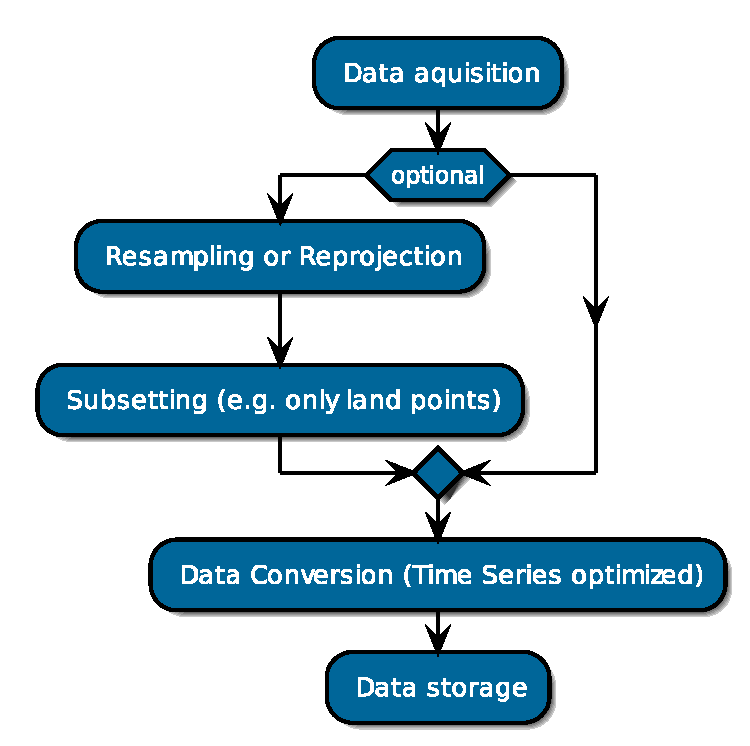
\includegraphics[width=0.20\textwidth]{graphics/preprocessing.eps}
      \end{tikzfigure}
      }
      
  \end{subcolumns}

    \figureblockoffset{}{
      \begin{tikzfigure}[Processing pipeline implemented in the pytesmo
        validation framework for comparing geospatial time series datasets. \label{fig:val_framework}]
          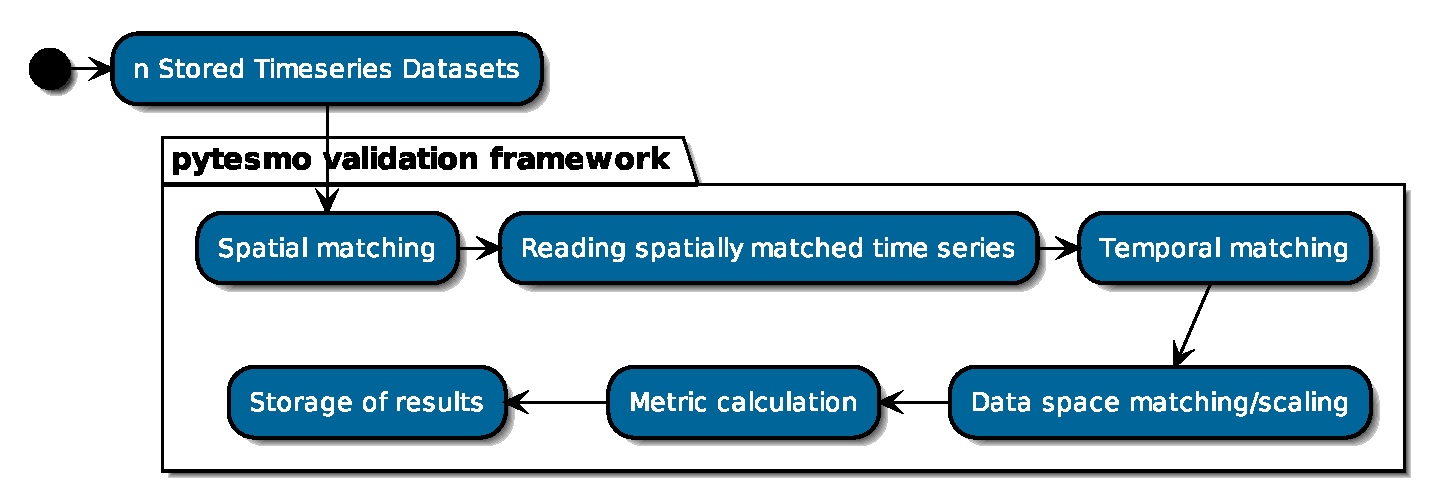
\includegraphics[width=0.40\textwidth]{graphics/validation_framework.eps}
      \end{tikzfigure}
      }

  
  \column{.5}

  
  \block{}{ 
    \begin{multicols} {2}

      Fig. \ref{fig:val_framework} shows the processing steps implemented in the
      pytesmo validation framework. First the n datasets are spatially matched
      to the defined spatial reference dataset. After this the time series at
      the spatially matched locations are read and temporally matched to the
      temporal reference dataset. An optional data space matching or scaling is
      performed against the scaling reference.


      The spatial, temporal and data space matched time series are then handed
      over to the metric calculators for the calculation of the supported
      metrics. These metric calculators are generally the only function that a
      user must implement to support a new metric. Metric calculators for common
      use cases are included in \code{pytesmo}. The calculated metrics are then
      returned and stored as netCDF files.

    \end{multicols}
    }

  
    \block{4. Processing SMAP data with \code{poets\degree}}{

      This Section will show an example of SMAP data processing from
      downloading the data to using it in a validation. The setup will be
      similar with other supported datasets.

      After installation of the \code{smap\_io} package the shell command
      \code{smap\_download} will be available. It downloads the SMAP data from
      the NASA servers and also supports authentification (not shown).

     \begin{tcolorbox}[colframe=tulightblue, arc=0mm]
     \label{lst:download_smap}
     \inputminted[bgcolor=light-gray]{bash}{download_smap.sh}
     \tcblower
     \captionof{listing}{Downloading SMAP SPL3SMP image data from 2016-01-01
       until 2016-02-01 with 4 parallel processes using the \code{smap\_io} package.}
     \end{tcolorbox}

     When the data is downloaded it can be read with the Python class \code{SPL3SMP\_Ds}:

     \begin{tcolorbox}[colframe=tulightblue, arc=0mm]
     \label{lst:read_smap}
     \inputminted[bgcolor=light-gray]{python}{read_smap.py}
     \tcblower
     \captionof{listing}{Reading SMAP SPL3SMP image data using the \code{smap\_io} package.}
     \end{tcolorbox}

     The images can then be converted into a time series optimized format using
     the command line program \code{smap\_repurpose}.

     \begin{tcolorbox}[colframe=tulightblue, arc=0mm]
     \label{lst:repurpose_smap}
     \inputminted[bgcolor=light-gray]{bash}{smap_repurpose.sh}
     \tcblower
     \captionof{listing}{Conversion of SMAP SPL3SMP image data into a time
       series format from 2016-01-01 to 2016-02-01 for the two variables
       soil\_moisture and soil\_moisture\_error.}
     \end{tcolorbox}

     The time series can the be read using the \code{SMAPTs} class as shown in
     Listing 4.

     \begin{tcolorbox}[colframe=tulightblue, arc=0mm]
     \inputminted[bgcolor=light-gray]{python}{read_smap_ts.py}
     \label{lst:read_smap_ts}
     \tcblower
     \captionof{listing}{Reading of the SMAP time series format produced by the
       \texttt{smap\_repurpose} command. The returned time series is a
       \texttt{pandas.DataFrame}.}
     \end{tcolorbox}

     Listing 5 shows how to use the converted data in the pytesmo validation
     framework together with GLDAS and ASCAT. More details about how the
     \texttt{process} is started, parallelized and how the results look like can
     be found in the documentation of the package.

     \begin{tcolorbox}[colframe=tulightblue, arc=0mm]
     \label{lst:validation}
     \inputminted[bgcolor=light-gray]{python}{validation_fwork.py}
     \tcblower
     \captionof{listing}{Setup of a global validation between SMAP, GLDAS and
       ASCAT without import statements. In this case SMAP will be the spatial
       reference, ASCAT the temporal matching reference and both SMAP and ASCAT
       will be scaled into the GLDAS data space using CDF matching. All
       combinations of the three datasets will be sent to the metrics
       calculatiors. In sets of 2 for the standard metrics like R or RMSD and in
       sets of 3 for triple collocation. }
     \end{tcolorbox}
    }

    \block{5. Usage and Contribution}{

      All information about the \code{poets\degree} project and its packages can
      be found on the website {\huge \link{http://tuw-geo.github.io/poets/}}


    }
\end{columns}

\end{document}
